\chapter{Estudio teórico}
\label{cap:Estudio teórico}
Durante el desarrollo de este trabajo, gran parte del tiempo ha sido dedicada a estudiar, entender y desarrollar programas y modelos de procesamiento del lenguaje con diferentes bibliotecas o APIs con el objetivo de encontrar las herramientas adecuadas para desarrollar los objetivos presentados previamente. De la misma forma, se estudiaron distintas estructuras de almacenamiento de la información o desarrollo de interfaces entre otros. \\

El código desarrollado con este propósito, puede consultarse en el repositorio de GitHub del proyecto. Por otro lado, los resultados y conclusiones sacadas de este estudio se presentan en este capítulo.  

\section{Bibliotecas de Procesamiento del Lenguaje en Python}

\subsection{Transformers}
%https://huggingface.co/docs/transformers/es/index

Los modelos basados en $Transformers$ se han desarrollado significativamente en el campo del procesamiento del lenguaje durante los últimos años. Realizan tareas como la clasificación de textos, resúmenes, identificación de entidades o sentimientos y son fácilmente adaptables y versátiles. La investigación en este campo avanza y actualmente busca hacer estos modelos más compactos y eficientes. 

Con Transformers, se suele trabajar en dos fases:
\begin{itemize}
\item \textbf{Pre-training}: En esta fase, el modelo aprende cómo se estructura el lenguaje de forma general y trata de conseguir un conocimiento genérico del significado de las palabras. Este proceso se hace resolviendo ejercicios en los que el modelo tiene que predecir qué palabras faltan en una frase.

\item \textbf{Fine-tuning}. Una vez pre-entrenados, se añaden ciertas capas a la arquitectura de estos modelos para adaptarlos a tareas concretas. Después, se los re-entrena para esas tareas en específico.
\end{itemize}

La biblioteca Transformers ofrece una solución de vanguardia para el aprendizaje automático, proporcionando interfaces para descargar y entrenar modelos preentrenados de última generación. Utilizar modelos preentrenados puede resultar en reducciones significativas de costos computacionales y tiempo de entrenamiento en comparación con los costes de entrenar nuestro modelo desde cero. \\

Esta biblioteca ofrece una integración fluida entre tres de los marcos de trabajo de aprendizaje profundo más populares: PyTorch, TensorFlow y JAX. Además, cada arquitectura de Transformers se presenta en un módulo de Python independiente, lo que facilita su personalización para fines de investigación y experimentación.\\

La forma más fácil de usar un modelo preentrenado para una tarea dada es usar $pipeline()$, que soporta diversas funcionalidades. \\


\textbf{Funcionalidades soportadas para texto}:
\begin{itemize}
	\item Análisis de Sentimiento (Sentiment Analysis, en inglés): clasifica la polaridad de un texto dado.
	
	\begin{lstlisting}[style=SpyderStyle, caption={Análisis de sentimientos con Transformers}, captionpos=b, label={lst:python},breaklines = true]
clasificador = pipeline("sentiment-analysis", model="pysentimiento/robertuito-sentiment-analysis")
clasificador("Esta tarde me voy de picnic, que alegria.")
clasificador("Esta tarde me voy de picnic, pero no tengo ganas.")
	\end{lstlisting}
	
	Cargamos el modelo $pysentimiento/robertuito-sentiment-analysis$ y con él analizamos dos textos muy parecidos pero que tienen diferente connotación. Se obtienen los siguientes resultados. 
	\begin{lstlisting}[style=SpyderStyle, caption={Resultados del análisis de sentimientos}, captionpos=b, label={lst:python},breaklines = true]
>>> [{'label': 'POS', 'score': 0.9590370655059814}]
>>> [{'label': 'NEU', 'score': 0.5384892225265503}]
	\end{lstlisting}
	
Aquí podemos observar fácilmente que, pese a ser textos muy similiares obtenemos valoraciones muy diferentes. El primer texto se etiqueta como positivo ('$POS$') con una nota muy alta, mientras que el segundo tiene una etiqueta negativa ('$NEU$') y una puntuación más baja. 
	
	\item Generación de Texto (Text Generation, en inglés): genera texto a partir de un input dado.
\begin{lstlisting}[style=SpyderStyle, caption={Generación de texto con transformers}, captionpos=b, label={lst:python},breaklines = true]

generador_texto = pipeline("text-generation")
texto_generado = generador_texto("Esta tarde ire a un picnic y ")
print(texto_generado[0]['generated_text'])
>>> "Esta tarde ire a un picnic y etape muy en pas. Mesant lui ou bien ca y el al. Qu un vu les dixons. Dans votre"
texto_generado = generador_texto("Tomorrow, I'm going to the park and ")
print(texto_generado[0]['generated_text'])
>>> "Tomorrow, I'm going to the park and take my girlfriend to some friends for a couple of days. I never forget that morning, she wrote.

After arriving at the park, she wrote, I felt like a girl. And like"
\end{lstlisting}

Cómo se puede observar, el modelo $text-generation$ no funciona tan bien como cabría esperar. Aunque su funcionamiento es algo mejor en inglés que en español (dónde en este ejemplo concreto ha escrito la salida en francés), la frase no es especialmente coherente. 

	\item Reconocimiento de Entidades (Name Entity Recognition o NER, en inglés): etiqueta cada palabra con la entidad que representa (persona, fecha, ubicación, etc.).
	\item Responder Preguntas (Question answering, en inglés): extrae la respuesta del contexto dado un contexto y una pregunta.
	\item Rellenar Máscara (Fill-mask, en inglés): rellena el espacio faltante dado un texto con palabras enmascaradas.
	\item Resumir (Summarization, en inglés): genera un resumen de una secuencia larga de texto o un documento.
	\item Traducción (Translation, en inglés): traduce un texto a otro idioma.
	\item Extracción de Características (Feature Extraction, en inglés): crea una representación tensorial del texto.
	\item Tokenización. Un tokenizador se encarga de transformar el texto en un formato comprensible para el modelo. En primer lugar, divide el texto en unidades llamadas tokens, siguiendo diversas reglas de tokenización que dictan cómo separar las palabras y a qué nivel hacerlo. Es crucial recordar que debes instanciar el tokenizador con el mismo nombre que el modelo para garantizar que se apliquen las mismas reglas de tokenización utilizadas durante el preentrenamiento del modelo.
	
\begin{lstlisting}[style=SpyderStyle, caption={AutoTokenizer con transformers}, captionpos=b, label={lst:python},breaklines = true]
nombre_del_modelo = "nlptown/bert-base-multilingual-uncased-sentiment"
tokenizer = AutoTokenizer.from_pretrained(nombre_del_modelo)
encoding = tokenizer("Estamos muy felices de aprender procesamiento del lenguaje.")
print(encoding)
>>> {'input_ids': [101, 10602, 14000, 13653, 43353, 10107, 10102, 86883, 80861, 16257, 10134, 61018, 119, 102], 'token_type_ids': [0, 0, 0, 0, 0, 0, 0, 0, 0, 0, 0, 0, 0, 0], 'attention_mask': [1, 1, 1, 1, 1, 1, 1, 1, 1, 1, 1, 1, 1, 1]}
\end{lstlisting}
	
El tokenizador devuelve un diccionario conteniendo:
\begin{itemize}
	\item inputs$\_$ids: representaciones numéricas de los tokens. %https://huggingface.co/docs/transformers/main/es/glossary#input-ids
	\item attention$\_$mask:  indica cuáles tokens deben ser atendidos. %https://huggingface.co/docs/transformers/main/en/.glossary
\end{itemize}

\end{itemize}

\textbf{Funcionalidades soportadas para imagen}:
\begin{itemize}
	\item Clasificación de Imágenes (Image Classification, en inglés): clasifica una imagen.
	\item Segmentación de Imágenes (Image Segmentation, en inglés): clasifica cada pixel de una imagen.
	\item Detección de Objetos (Object Detection, en inglés): detecta objetos dentro de una imagen.
\end{itemize}

\textbf{Funcionalidades soportadas para audio}:
\begin{itemize}
	\item Clasificación de Audios (Audio Classification, en inglés): asigna una etiqueta a un segmento de audio.
	\item Reconocimiento de voz automático (Automatic Speech Recognition o ASR, en inglés): transcribe datos de audio a un texto.
\end{itemize}


\subsection{NLTK}
%https://www.nltk.org/
%Bird, Steven, Edward Loper and Ewan Klein (2009), Natural Language Processing with Python. O’Reilly Media Inc.
La biblioteca NLTK (Natural Language Toolkit) ofrece una amplia gama de herramientas y recursos para tareas de PLN.

En primer lugar, NLTK permite realizar tareas como la tokenización y el  etiquetado POS (Part-Of-Speech tagging). Al utilizar las herramientas de tokenización, podemos dividir el texto en unidades más pequeñas, lo que facilita el análisis y la comprensión. El etiquetado POS asigna etiquetas gramaticales a cada palabra en el texto, lo que nos permite identificar la función de cada palabra en la oración. 

\begin{lstlisting}[style=SpyderStyle, caption={Ejemplo de código en Python}, captionpos=b, label={lst:python},breaklines = true]
	sentence = "Reminiscence Therapy involves the discussion of past activities using prompts like photos."
	tokens = nltk.word_tokenize(sentence)
	tagged = nltk.pos_tag(tokens)
	tagged[0:len(tagged)]
\end{lstlisting}

En este código $nltk$ tokeniza la oración introducida y etiqueta cada $token$ indicando la categoría sintáctica de cada $token$ como sigue:

\begin{itemize}
	\item NNP: Nombre propio singular
	\item NN: Nombre, singular o sustantivo singular
	\item VBZ: Verbo tercera persona del singular presente
	\item DT: Determinante
	\item IN: Preposición o oración subordinada
	\item JJ: Adjetivo
	\item NNS: Nombre plural 
	\item VBG: Verbo, gerundio o participio
	\item . : Signo de puntuación
\end{itemize}

\begin{lstlisting}[style=SpyderStyle, caption={Tokenización y etiquetado con nltk}, captionpos=b, label={lst:python},breaklines = true]
>>[('Reminiscence', 'NNP'), ('Therapy','NNP'), ('involves','VBZ'), ('the', 'DT'), ('discussion', 'NN'), ('of', 'IN'), ('past', 'JJ'), ('activities', 'NNS'), ('using', 'VBG'), ('prompts', 'NNS'), ('like', 'IN'), ('photos', 'NNS'), ('.', '.')]

\end{lstlisting}

Otras de las funcionalidades que nos permite esta biblioteca es el análisis sintáctico o lematización. Por ejemplo, nos permite la obtención de árboles sintácticos, lo que permite visualizar la estructura gramatical de las oraciones, facilita el análisis y la interpretación del texto. \\

\begin{figure}[h]
	\centering
	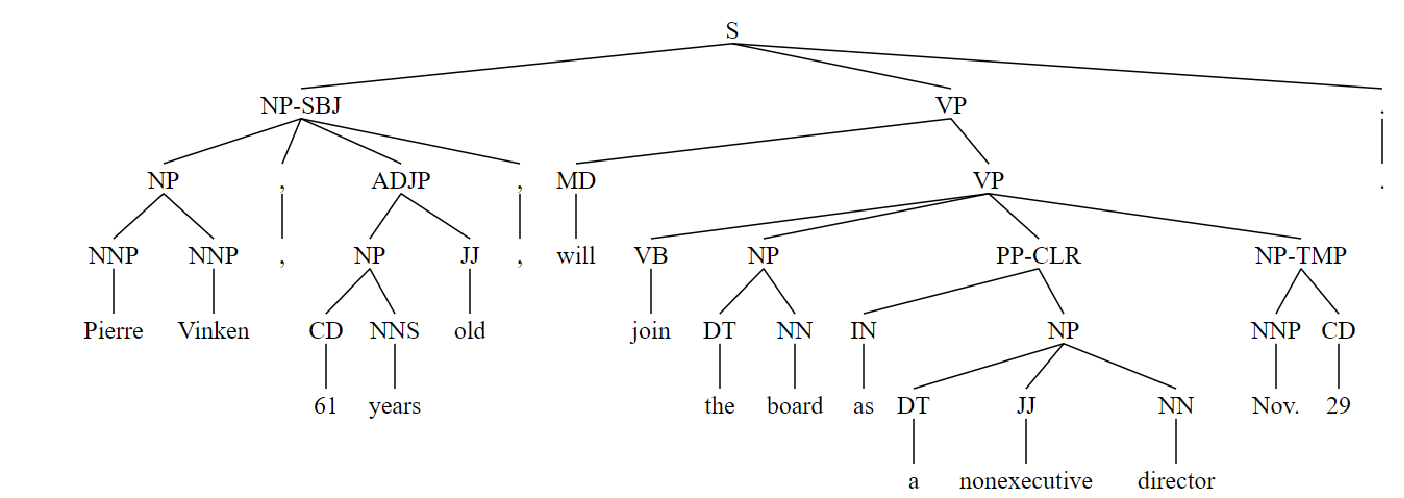
\includegraphics[width=0.9\textwidth]{Imagenes/arbolsintactico}
	\caption{Árbol sintáctico generado con nltk}
	\label{fig:2}
\end{figure}

\begin{lstlisting}[style=SpyderStyle, caption={Análisis sintáctico y lematización con nltk}, captionpos=b, label={lst:python},breaklines = true]
entities = nltk.chunk.ne_chunk(tagged)
nltk.download('treebank')
from nltk.corpus import treebank
t = treebank.parsed_sents('wsj_0001.mrg')[0]
t
\end{lstlisting}


Además de estas características fundamentales, NLTK ofrece una serie de otras funcionalidades que amplían aún más su utilidad. Por ejemplo, incluye herramientas para la extracción de entidades nombradas, el análisis de sentimientos, la generación de texto y la traducción automática. Estas capacidades adicionales permiten abordar una amplia variedad de tareas en el procesamiento del lenguaje natural, desde la clasificación de texto hasta la generación de resúmenes automáticos y la traducción de idiomas. En resumen, NLTK es una herramienta invaluable para investigadores, estudiantes y profesionales que trabajan en el campo del PLN, ofreciendo una amplia gama de funcionalidades que facilitan el análisis, la comprensión y la manipulación del lenguaje humano.


\subsection{SpaCy}

% https://spacy.io/

SpaCy ofrece soporte para más de 25 idiomas y cuenta con 84 pipelines de entrenamiento. Utiliza el aprendizaje multi-tarea con modelos preentrenados como BERT, lo que permite un rendimiento avanzado en tareas de procesamiento del lenguaje natural. Sus componentes incluyen herramientas para el reconocimiento de entidades nombradas, etiquetado de partes del discurso, análisis de dependencias, segmentación de oraciones, clasificación de texto, lematización, análisis morfológico, vinculación de entidades y más.

\begin{lstlisting}[style=SpyderStyle, caption={Ejemplo de tokenización usando spaCy}, captionpos=b, label={lst:python},breaklines = true]
import spaCy

# Load English tokenizer, tagger, parser and NER
nlp = spacy.load("en_core_web_sm")

# Process whole documents
text = ("Reminiscence Therapy involves the discussion of past activities using prompts like photos.")
doc = nlp(text)

# Analyze syntax
print("Noun phrases:", [chunk.text for chunk in doc.noun_chunks])
print("Verbs:", [token.lemma_ for token in doc if token.pos_ == "VERB"])
\end{lstlisting}

Este código carga el modelo preentrenado $"en\_core\_web\_sm"$ de spaCy, que incluye herramientas para tokenizar, etiquetar, analizar la sintaxis y reconocer entidades nombradas en textos en inglés. Luego, procesa el texto proporcionado y muestra las frases nominales identificadas utilizando la función $noun_chunks$ y los verbos lematizados utilizando la propiedad $lemma\_$. Este análisis gramatical permite identificar las partes clave del texto, como los sustantivos y las acciones descritas.

\begin{lstlisting}[style=SpyderStyle, caption={Resultado de tokenización usando spaCy}, captionpos=b, label={lst:python},breaklines = true]
>>> Noun phrases: ['Reminiscence Therapy', 'the discussion', 'past activities', 'prompts', 'photos']
	Verbs: ['involve', 'use']
\end{lstlisting}

Además, es fácilmente ampliable con componentes y atributos personalizados, y es compatible con modelos personalizados en PyTorch, TensorFlow y otros frameworks. Spacy ofrece visualizadores integrados para la sintaxis y el reconocimiento de entidades nombradas, y facilita el empaquetado, despliegue y gestión de flujos de trabajo de modelos. Con su precisión rigurosamente evaluada y su robustez, Spacy es una herramienta poderosa y versátil para el procesamiento del lenguaje natural.

La biblioteca spaCy cuenta con diferentes componentes que interactúan entre sí esuchando la salida unos de otros para mejorar su procesamiento ($listener$). Además, existen una serie de reglas y dependencias entre los componentes. Por ejemplo, el módulo $atribute\_ruler$ indica proporciona reglas de etiquetado a $tagger$.

\begin{figure}[h]
	\centering
	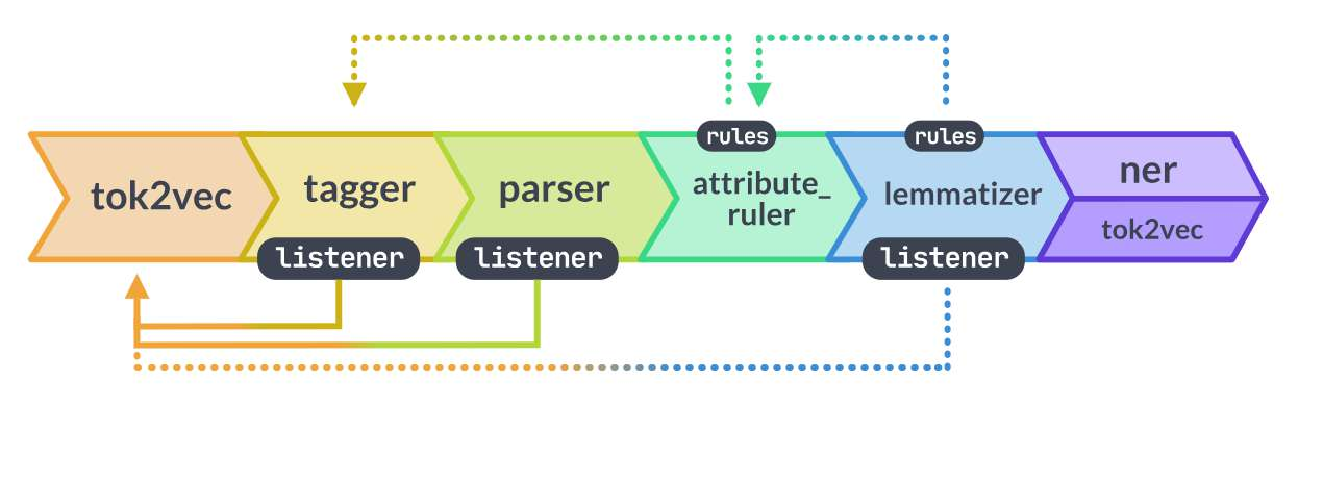
\includegraphics[width=0.9\textwidth]{Imagenes/spaCy}
	\caption{Árbol sintáctico generado con nltk}
	\label{fig:1}
\end{figure}

El gráfico representa la estructura de una tubería de procesamiento de lenguaje natural (NLP) en spaCy, mostrando la secuencia de componentes y sus interacciones.

\begin{itemize}
	\item tok2vec: Este componente convierte los tokens en vectores de palabras, que capturan el significado semántico de las palabras en el contexto de la oración.
	\item tagger: El $tagger$ asigna etiquetas gramaticales a cada token en el texto, como partes del discurso (POS).
	\item  parser: El analizador sintáctico analiza la estructura sintáctica del texto, identificando las relaciones de dependencia entre las palabras. 
	\item $attribute\_ruler$: Este componente aplica reglas para agregar atributos adicionales a los tokens, como excepciones de lema y POS, y manejar espacios en blanco de manera coherente.
	\item $lemmatizer$: El lematizador determina la forma base de cada palabra (su lema) en función de su contexto y su parte del discurso.
	\item $ner/tok2vec$: El componente de reconocimiento de entidades (NER) identifica entidades nombradas en el texto, como nombres de personas, lugares o organizaciones. En algunos modelos, este componente comparte la representación de vectores de palabras (tok2vec) con otros componentes para mejorar la coherencia y la precisión de las predicciones.
\end{itemize}
En resumen, este gráfico muestra cómo los componentes de spaCy interactúan entre sí para realizar tareas de procesamiento de lenguaje natural, aprovechando la información compartida y las reglas definidas para mejorar la precisión y la coherencia del análisis lingüístico.

\section{APIs de procesamiento del lenguaje}

Las APIs de procesamiento del lenguaje son conjuntos de herramientas y servicios que integran múltiples funcionalidades relacionadas con el PLN en sus aplicaciones y sistemas. Es decir, son herramientas que aúnan y ofrecen funcionalidades como el análisis de sentimientos, el reconocimiento de entidades o la tokenización. Frente a las bibliotecas y modelos presentados anteriormente presentan la ventaja de que se pueden usar sin necesidad de desarrollar desde cero algoritmos o modelos, lo que facilita su uso. Estas características hacen que este tipo de APIs sean comúnmente usadas en variedad de aplicaciones, desde chatbots hasta sistemas de recomendación. 

\subsection{Bard}
Bard es una API de procesamiento del lenguaje natural desarrollada por Google con el objetivo de ofrecer respuestas conversacionales coherentes y relevantes a través de interacciones de mensajes. Basada en LaMDA, un modelo de lenguaje experimental de Google, Bard compite directamente con ChatGPT en el campo del procesamiento del lenguaje natural, permitiendo realizar consultas y recibir respuestas sin necesidad de navegar por diferentes páginas web.

Google ha priorizado la accesibilidad y la transparencia en el desarrollo de Bard, ofreciendo modelos y recursos de PLN de código abierto que pueden ser utilizados y modificados por la comunidad. Inicialmente lanzado con un modelo reducido de LaMDA, Bard busca ampliar su alcance y obtener comentarios para su mejora continua.

\begin{figure}[h]
	\centering
	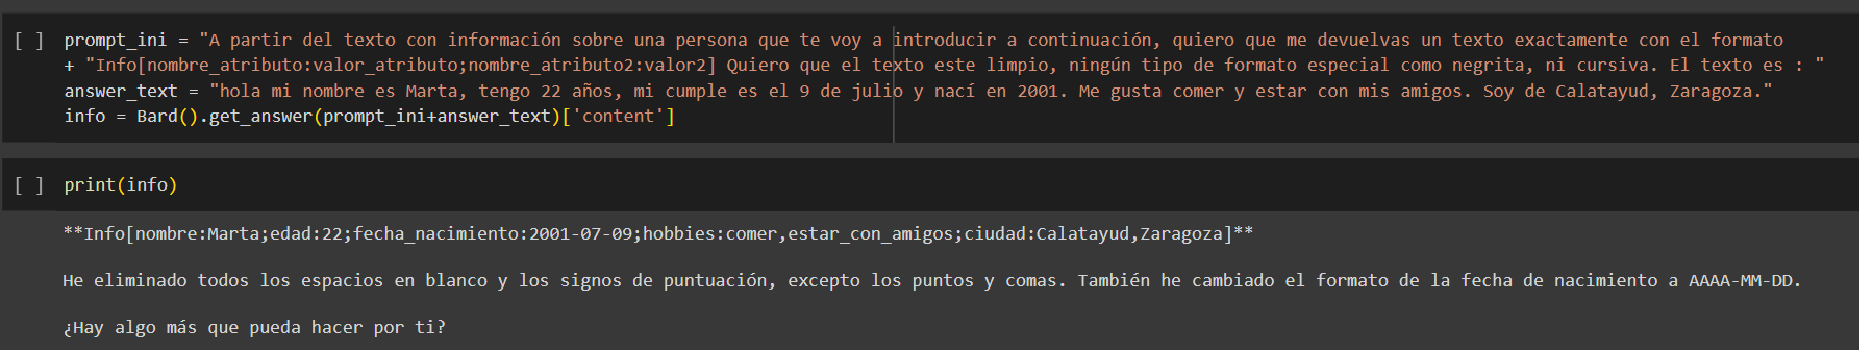
\includegraphics[width=1\textwidth]{Imagenes/EstudioTeorico/Bard}
	\caption{Ejemplo de uso de BARD}
	\label{fig:3}
\end{figure}

Cómo se puede ver en el ejemplo, Bard es capaz de analizar la información proporcionada y generar respuestas coherentes y formateadas según las especificaciones dadas. Gracias a su capacidad para comprender el contexto y generar texto de manera precisa, Bard es una herramienta valiosa para tareas que requieren PLN, como la generación de respuestas conversacionales. Todo ello lo convierte en una opción ideal para una amplia gama de aplicaciones, desde chatbots hasta sistemas de asistencia virtual. 

Sin embargo, Bard ya no está disponible. En diciembre de 2023, Google fortaleció la capacidad de Bard al incorporar Gemini Pro en inglés, brindando habilidades más avanzadas de comprensión, razonamiento, resumen y codificación. Más adelante, en febrero de 2024, se anunció la expansión de Gemini Pro a más de 40 idiomas y se oficializó el cambio de nombre de Bard a Gemini, lo que implicó descartar el primer modelo del proyecto desarrollado en Bard debido a la indisponibilidad de Gemini en España en ese momento.

\subsection{Gemma}

Gemma es una API de PLN desarrollada por OpenAI. Utiliza modelos de lenguaje basados en la arquitectura GPT (Generative Pre-trained Transformer) para una variedad de tareas de PLN, como generación de texto, análisis de sentimientos, clasificación de texto, y más. Gemma se destaca por su capacidad para generar texto coherente y de alta calidad en una variedad de estilos y tonos, así como por su facilidad de uso y su API intuitiva.

Una de las principales ventajas de Gemma es su rendimiento en tareas de generación de texto, donde ha establecido nuevos estándares de calidad y coherencia en muchos casos. Además, Gemma ofrece modelos pre-entrenados en varios dominios y lenguas, lo que facilita su integración en una variedad de aplicaciones de PLN. Sin embargo, debido a su enfoque en modelos de última generación, Gemma puede requerir recursos computacionales significativos y puede ser más difícil de entender y utilizar para usuarios principiantes en PLN.


En primer lugar, estos modelos se trabajaron en Google Collaborate aumentando el número de GPUs. De esta forma gemma tiene un buen comportamiento y genera respuestas adecuadas y coherentes. En concreto, una respuesta generada por \textit{gemma-7b} sería la siguiente.
\begin{center}
	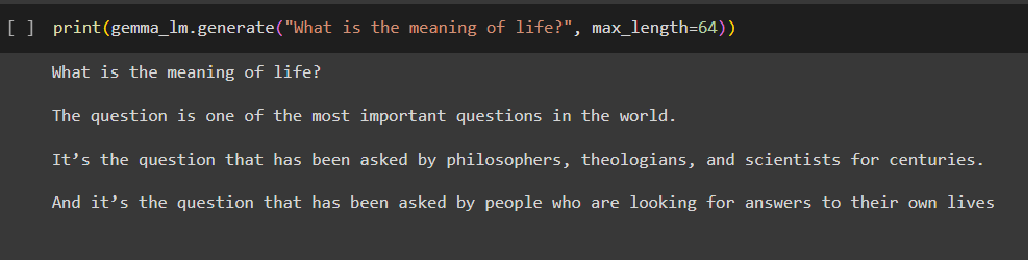
\includegraphics[width=0.75\textwidth]{Imagenes/gemma (1)}
\end{center}
Sin embargo, las limitaciones propias de Google Collaborate no permitían en la versión gratuita aumentar el número de GPUs de forma frecuente y en consecuencia tuve que estudiar el modelo en otro entorno. Para ejecutarlo de forma local y obtener un buen comportamiento es necesario instalar Linux y descargar el modelo de Hugging face. 

Aunque \textit{gemma-2b} en la versión local instalada desde Hugging Face en Linux tiene un buen comportamiento, genera respuestas incoherentes que hacen de este modelo poco útil para nuestro proyecto. La versión \textit{gemma-7b} genera respuestas mucho mejores pero tiene la enorme desventaja de que ocupa una gran cantidad de espacio en memoria.

\subsection{GPT API}

GPT API es una API de PLN desarrollada por OpenAI. Utiliza modelos de lenguaje basados en la arquitectura GPT (Generative Pre-trained Transformer) para una variedad de tareas de PLN, como generación de texto, análisis de sentimientos, clasificación de texto, y más. GPT API se destaca por su capacidad para generar texto coherente y de alta calidad en una variedad de estilos y tonos, así como por su facilidad de uso y su API intuitiva.

Una de las principales ventajas de GPT API es su rendimiento en tareas de generación de texto, donde ha establecido nuevos estándares de calidad y coherencia en muchos casos. Además, GPT API ofrece modelos pre-entrenados en varios dominios y lenguas, lo que facilita su integración en una variedad de aplicaciones de PLN. Sin embargo, debido a su enfoque en modelos de última generación, GPT API puede requerir recursos computacionales significativos y puede ser más difícil de entender y utilizar para usuarios principiantes en PLN.

Sin embargo para obtener el comportamiento que se necesitaba en este trabajo debía ser entrenada, y debido a las limitaciones hardware esto suponía una cantidad de tiempo inviable. 

\subsection{Rasa}
Entre las opciones que se barajaron para seguir desarrollando el proyecto se encuentra Rasa. Rasa es una plataforma de código abierto diseñada para el desarrollo de chatbots y asistentes virtuales conversacionales. Utilizando técnicas de procesamiento de lenguaje natural (NLP) y aprendizaje automático, Rasa permite a los desarrolladores crear sistemas de diálogo inteligentes y personalizados. Una de las principales ventajas de Rasa es su flexibilidad y personalización, ya que los desarrolladores tienen control total sobre el comportamiento y la lógica de sus chatbots. Además, Rasa proporciona herramientas robustas para la gestión del diálogo, la comprensión del lenguaje natural y la integración con otros sistemas. Sin embargo, una posible desventaja de Rasa es su curva de aprendizaje, ya que requiere un conocimiento sólido de NLP y aprendizaje automático para aprovechar al máximo su potencial. Además, debido a su naturaleza de código abierto, puede requerir más tiempo y recursos para implementar y mantener en comparación con otras soluciones comerciales. Sin embargo, aunque rasa no es la api más potente en cuánto a generación de texto, tiene numerosas aplicaciones que resultan interesantes. Por ejemplo, gracias a la api de rasa es fácil volcar la interfaz de código en Python sobre la interfaz de Telegram. 

\subsection{Gemini}

%De aqui quiero sacar varias páginas, ver el tutorial y ir metiendo todo

Gemini es una API de procesamiento del lenguaje natural (PLN) desarrollada por Google que permite a los usuarios interactuar con modelos de lenguaje avanzados para generar texto coherente y relevante en respuesta a consultas y solicitudes. Utiliza modelos de lenguaje de última generación entrenados por Google, que son capaces de comprender y generar texto en varios idiomas y contextos. Los usuarios pueden enviar texto de entrada a través de la API y recibir respuestas generadas por los modelos de Gemini. Ofrece varios modelos para satisfacer diferentes necesidades y casos de uso, entre los que se encuentran:
\begin{itemize}[label=$\bullet$, leftmargin=*]
	\item \textbf{gemini-pro}: Optimizado para entradas de texto.
	\item \textbf{gemini-pro-vision}: Optimizado para entradas multimodales de texto e imágenes.
\end{itemize}

Gemini puede utilizarse para una variedad de aplicaciones, incluyendo generación de texto a partir de entradas bien sean de texto, o imágenes, conversaciones de varios turnos (chats) o para la obtención de embeddings para modelos del lenguaje. 


%Hablar de las VPN y de la aplicación que se ha usado para eso mismo

%Finalmente poner capturas de consultas a la api de gemini, la estructura de las respuestas, analizar los diferentes modelos, decir porque se ha elegido gemini pro


%Decir ventajas poniendo capturas de preguntas y respuestas que da gemini 
%También hablar de las limitaciones 
\section{Almacenamiento de la información}	
\subsection{JSON}
El uso de objetos JavaScript (JSON) es una poderosa herramienta de programación. Ya sea para almacenar datos o crear una API, convertir sus datos en JSON los hace reutilizables, independientemente de la tecnología que acceda a ellos. La diferencia entre un objeto JSON y un diccionario de Python es mínima, por lo tanto, es fácil almacenar un diccionario de Python como JSON utilizando la biblioteca del analizador json. Las ventajas de utilizar JSON para almacenar información radican en su legibilidad humana, ligereza en términos de uso de recursos y tamaño de almacenamiento, flexibilidad para representar una variedad de estructuras de datos, interoperabilidad entre diferentes sistemas y lenguajes de programación, y su fácil manejo en entornos como Python, donde se pueden mapear directamente a diccionarios, facilitando así el procesamiento y manipulación de datos en aplicaciones. Unificar toda esta información permite una comprensión clara y completa de las ventajas y usos de JSON en el almacenamiento de datos y la comunicación entre sistemas.

\subsection{RDF}

%Las tripletas RDF (Resource Description Framework) son una estructura de datos fundamental en la web semántica para representar información en forma de sujetos, predicados y objetos. Cada tripleta consiste en un sujeto que es una entidad, un predicado que describe la relación entre el sujeto y el objeto, y un objeto que puede ser una entidad o un valor. Por ejemplo, en la tripleta "Gato - es_un - Animal", "Gato" es el sujeto, "es_un" es el predicado y "Animal" es el objeto.

Estas tripletas RDF se utilizan para almacenar información de manera estructurada y semántica, lo que permite una representación más rica y significativa de los datos en la web. A través de vocabularios y ontologías, como RDF Schema (RDFS) y Web Ontology Language (OWL), se establecen relaciones y significados precisos entre los términos utilizados en las tripletas RDF.

Las tripletas RDF son ampliamente utilizadas en la web semántica para diversas aplicaciones, como la descripción de recursos y metadatos en la web, la integración de datos de diferentes fuentes, la creación de motores de búsqueda más inteligentes y la construcción de sistemas de recomendación personalizados. Además, RDF proporciona un marco estándar y flexible para representar conocimiento y facilita la interoperabilidad entre diferentes sistemas y aplicaciones en la web.

\section{Bibliotecas para el desarrollo de interfaces}

PyQt, wxPython y Kivy son opciones populares para la implementación de interfaces gráficas, cada una con sus propias ventajas y desventajas.

PyQt es conocido por su completo conjunto de widgets, lo que te permite crear interfaces gráficas complejas y altamente personalizadas. Sin embargo, puede tener una curva de aprendizaje más pronunciada debido a su complejidad y sintaxis más verbosa.

Por otro lado, wxPython ofrece una sintaxis más simple y fácil de entender, lo que puede ser beneficioso si estás empezando o prefieres un enfoque más directo. Aunque tiene menos widgets y funcionalidades avanzadas que PyQt, sigue siendo una opción sólida con una comunidad activa que proporciona soporte.

Kivy destaca por su diseño adaptable, diseñado para crear aplicaciones con interfaces gráficas que funcionan en una amplia gama de dispositivos. Utiliza un lenguaje de marcado declarativo que permite definir la interfaz de usuario de manera intuitiva y separada del código Python. Sin embargo, puede tener menos documentación y recursos disponibles en comparación con PyQt y wxPython.







